\section[dt]{Decision Tree / Model complexity}

\begin{frame}[fragile]
\frametitle{How does a Decision Tree work?}

\begin{center}
\begin{tikzpicture}   
\draw[draw=none] (-4,1.5) rectangle (4,-3.5);

\draw<2> (0,0) node[hbox] (N1) {$x < 0$};
\draw<1,3->(0,0) node[box=white] (N1) {$x < 0$};

\draw (-2,-1) node[box=tree300] (N2) {$y < 0$};

\draw<3> (2,-1) node[hbox] (N3) {$x < 4$};
\draw<1-2,4-5> (2,-1) node[box=tree700] (N3) {$x < 4$};

\draw[->,line width=1pt,black] (N1.south) -> (N2.north);
\draw[->,line width=1pt,black] (N1.south) -> (N3.north);
\draw (-3,-2) node[box=tree200] (N4) {$x < -5$};
\draw (-1,-2) node[box=tree400] (N5) {$y < 3$};

\draw<4> (1,-2) node[hbox] (N6) {$y < 0$};
\draw<1-3,5> (1,-2) node[box=tree600] (N6) {$y < 0$};

\draw (3,-2) node[box=tree800] (N7) {$x < 8$};
\draw[->,line width=1pt,black] (N2.south) -> (N4.north);
\draw[->,line width=1pt,black] (N2.south) -> (N5.north);
\draw[->,line width=1pt,black] (N3.south) -> (N6.north);
\draw[->,line width=1pt,black] (N3.south) -> (N7.north);
\draw (-3.5,-3) node[box=tree100] (N8) {$0.1$};
\draw (-2.5,-3) node[box=tree200] (N9) {$0.2$};
\draw (-1.5,-3) node[box=tree300] (N10) {$0.3$};
\draw (-0.5,-3) node[box=tree800] (N11) {$0.8$};
\draw (0.5,-3) node[box=tree400] (N12) {$0.4$};

\draw<5> (1.5,-3) node[hbox] (N13) {$0.7$};
\draw<1-4> (1.5,-3) node[box=tree700] (N13) {$0.7$};

\draw (2.5,-3) node[box=tree500] (N14) {$0.5$};
\draw (3.5,-3) node[box=tree900] (N15) {$0.9$};
\draw[->,line width=1pt,black] (N4.south) -> (N8.north);
\draw[->,line width=1pt,black] (N4.south) -> (N9.north);
\draw[->,line width=1pt,black] (N5.south) -> (N10.north);
\draw[->,line width=1pt,black] (N5.south) -> (N11.north);
\draw[->,line width=1pt,black] (N6.south) -> (N12.north);
\draw[->,line width=1pt,black] (N6.south) -> (N13.north);
\draw[->,line width=1pt,black] (N7.south) -> (N14.north);
\draw[->,line width=1pt,black] (N7.south) -> (N15.north);
\node[box=tree1000,opacity=.3,text opacity=1] at (-3.5,0.8) {$\begin{array}{c}x = 2 \\ y = 5\end{array}$};

\draw<2> node[box=tree500,opacity=.2,text opacity=1, text centered] at (0,1) {Is $x$ negative?};
\draw<3> node[box=tree500,opacity=.2,text opacity=1, text centered] at (0,1) {Is $x$ smaller than $4$?};
\draw<4> node[box=tree500,opacity=.2,text opacity=1, text centered] at (0,1) {Is $y$ negative?};
\draw<5> node[box=tree500,opacity=.2,text opacity=1, text centered] at (0,1) {Returned probability is $0.7$};

\end{tikzpicture}
\end{center}

\end{frame}

\begin{frame}[fragile]
\frametitle{How is a Decision Tree built?}

\begin{center}
\begin{tikzpicture}
\draw[draw=none] (-4,1.5) rectangle (4,-3.5);
\coordinate (start) at (0, 1);

  \draw<3> (0,0) node[hbox] (N1) {$x < 0$};
  \draw<4-> (0,0) node[box=tree500] (N1) {$x < 0$};
  \draw<2> (0,0) node[hbox] (N1) {\hphantom{$x < 0$}};
  \draw<1> (0,0) node[box=tree500] (N1) {\hphantom{$x < 0$}};

  \draw<5> (-2,-1) node[hbox] (N2) {$y < 0$};
  \draw<6-> (-2,-1) node[box=tree300] (N2) {$y < 0$};
  \draw<4> (-2,-1) node[hbox] (N2) {\hphantom{$y < 0$}};
  \draw<1-3> (-2,-1) node[box=tree500] (N2) {\hphantom{$y < 0$}};

    \draw<6-> (2,-1) node[box=tree700] (N3) {$x < 4$};
    \draw<6-> (-3,-2) node[box=tree200] (N4) {$x < -5$};
    \draw<6-> (-1,-2) node[box=tree400] (N5) {$y < 3$};
    \draw<6-> (1,-2) node[box=tree600] (N6) {$y < 0$};
    \draw<6-> (3,-2) node[box=tree800] (N7) {$x < 8$};
    \draw<1-5> (2,-1) node[box=tree500] (N3) {\hphantom{$x < 4$}};
    \draw<1-5> (-3,-2) node[box=tree500] (N4) {\hphantom{$x < -5$}};
    \draw<1-5> (-1,-2) node[box=tree500] (N5) {\hphantom{$y < 3$}};
    \draw<1-5> (1,-2) node[box=tree500] (N6) {\hphantom{$y < 0$}};
    \draw<1-5> (3,-2) node[box=tree500] (N7) {\hphantom{$x < 8$}};

\draw[->,line width=1pt,black] (N1.south) -> (N2.north);
\draw[->,line width=1pt,black] (N1.south) -> (N3.north);
\draw[->,line width=1pt,black] (N2.south) -> (N4.north);
\draw[->,line width=1pt,black] (N2.south) -> (N5.north);
\draw[->,line width=1pt,black] (N3.south) -> (N6.north);
\draw[->,line width=1pt,black] (N3.south) -> (N7.north);

    \draw<7-> (-3.5,-3) node[box=tree100] (N8) {$0.1$};
    \draw<7-> (-2.5,-3) node[box=tree200] (N9) {$0.2$};
    \draw<7-> (-1.5,-3) node[box=tree300] (N10) {$0.3$};
    \draw<7-> (-0.5,-3) node[box=tree800] (N11) {$0.8$};
    \draw<7-> (0.5,-3) node[box=tree400] (N12) {$0.4$};
    \draw<7-> (1.5,-3) node[box=tree700] (N13) {$0.7$};
    \draw<7-> (2.5,-3) node[box=tree500] (N14) {$0.5$};
    \draw<7-> (3.5,-3) node[box=tree900] (N15) {$0.9$};

    \draw<1-6> (-3.5,-3) node[box=tree500] (N8) {\hphantom{$0.1$}};
    \draw<1-6> (-2.5,-3) node[box=tree500] (N9) {\hphantom{$0.2$}};
    \draw<1-6> (-1.5,-3) node[box=tree500] (N10) {\hphantom{$0.3$}};
    \draw<1-6> (-0.5,-3) node[box=tree500] (N11) {\hphantom{$0.8$}};
    \draw<1-6> (0.5,-3) node[box=tree500] (N12) {\hphantom{$0.4$}};
    \draw<1-6> (1.5,-3) node[box=tree500] (N13) {\hphantom{$0.7$}};
    \draw<1-6> (2.5,-3) node[box=tree500] (N14) {\hphantom{$0.5$}};
    \draw<1-6> (3.5,-3) node[box=tree500] (N15) {\hphantom{$0.9$}};

\draw[->,line width=1pt,black] (N4.south) -> (N8.north);
\draw[->,line width=1pt,black] (N4.south) -> (N9.north);
\draw[->,line width=1pt,black] (N5.south) -> (N10.north);
\draw[->,line width=1pt,black] (N5.south) -> (N11.north);
\draw[->,line width=1pt,black] (N6.south) -> (N12.north);
\draw[->,line width=1pt,black] (N6.south) -> (N13.north);
\draw[->,line width=1pt,black] (N7.south) -> (N14.north);
\draw[->,line width=1pt,black] (N7.south) -> (N15.north);


\only<2>{
\draw node[box=tree500,opacity=.2,text opacity=1, text centered] at (0,1) {Search best-cut in complete dataset};
\draw [<->,thick] (4.5,0.5) node (yaxisx) [above] {$f$}
        |- (7,-1) node (xaxisx) [right] {$x$};
\coordinate (c) at (5.65,0.3);
\draw [black] plot [smooth] coordinates {(4.5,-1) (c) (6.8,-1)};

\draw [<->,thick] (4.5,-1.5) node (yaxisy) [above] {$f$}
        |- (7,-3) node (xaxisy) [right] {$y$};
\draw [black] plot [smooth] coordinates {(4.5,-3) (5,-2.4) (6.8,-3)};
}

\only<3>{
\node[box=tree500,opacity=.2,text opacity=1, text centered] at (0,1) {Best cut is $x < 0$};
\draw [<->,thick] (4.5,0.5) node (yaxisx) [above] {$f$}
        |- (7,-1) node (xaxisx) [right] {$x$};
\coordinate (c) at (5.65,0.3);
\draw [black] plot [smooth] coordinates {(4.5,-1) (c) (6.8,-1)};
\draw[dashed] (yaxisx |- c) node[left] {$f_{\textrm{max}}$}
        -| (xaxisx -| c) node[below] {best cut};
\fill[red] (c) circle (2pt);

\draw [<->,thick] (4.5,-1.5) node (yaxisy) [above] {$f$}
        |- (7,-3) node (xaxisy) [right] {$y$};
\draw [black] plot [smooth] coordinates {(4.5,-3) (5,-2.4) (6.8,-3)};
}

\only<4>{
\node[box=tree500,opacity=.2,text opacity=1, text centered] at (0,1) {Search best cut in dataset with $x < 0$};
\draw [<->,thick] (4.5,0.5) node (yaxisx) [above] {$f$}
        |- (7,-1) node (xaxisx) [right] {$x$};
\draw [black] plot [smooth] coordinates {(4.5,-1) (6,-0.4) (6.8,-1)};

\draw [<->,thick] (4.5,-1.5) node (yaxisy) [above] {$f$}
        |- (7,-3) node (xaxisy) [right] {$y$};
\coordinate (c) at (5.65,-1.8);
\draw [black] plot [smooth] coordinates {(4.5,-3) (c) (6.8,-3)};
}

\only<5>{
\node[box=tree500,opacity=.2,text opacity=1, text centered] at (0,1) {Best cut is $y < 0$};
\draw [<->,thick] (4.5,0.5) node (yaxisx) [above] {$f$}
        |- (7,-1) node (xaxisx) [right] {$x$};
\draw [black] plot [smooth] coordinates {(4.5,-1) (6,-0.4) (6.8,-1)};

\draw [<->,thick] (4.5,-1.5) node (yaxisy) [above] {$f$}
        |- (7,-3) node (xaxisy) [right] {$y$};
\coordinate (c) at (5.65,-1.8);
\draw [black] plot [smooth] coordinates {(4.5,-3) (c) (6.8,-3)};

\draw[dashed] (yaxisy |- c) node[left] {$f_{\textrm{max}}$}
        -| (xaxisy -| c) node[below] {best cut};
\fill[red] (c) circle (2pt);
}

\only<6>{
\node[box=tree500,opacity=.2,text opacity=1, text centered] at (0,1) {Repeat until tree is completed};
}

\only<7>{
\node[box=tree500,opacity=.2,text opacity=1, text centered] at (0,1) {Calculate purity in each leaf};
}

\end{tikzpicture}
\end{center}

\end{frame}


\begin{frame}
    \frametitle{Decision Tree}
    \begin{center}
      \begin{itemize}
              \item Classifies using a number of consecutive rectangular cuts 
              \item Each cut locally maximizes a separation gain measure
              \item Signal probability given by the purity in each leaf
              \item Interpretable (white box) model
      \end{itemize}
      \vspace{0.5em}
        \begin{tikzpicture}
            \node[anchor=south west,inner sep=0] (image) at (0,0) {\includegraphics[width=0.6\textwidth]{reg_tree_visualization.png}};
        \end{tikzpicture}
    \end{center}
\end{frame}

\begin{frame}
    \frametitle{Complete Decision Tree}
    \begin{center}
        \begin{tikzpicture}
            \node[anchor=south west,inner sep=0] at (0,0) {\includegraphics[width=0.6\textwidth]{tree_visualization.png}};
        \end{tikzpicture}


        \large{Complete tree with pure leaves $\rightarrow$ Complex model}


        \begin{tikzpicture}
            \node[anchor=north west,inner sep=0] at (0,0) {\includegraphics[width=0.6\textwidth]{tree_classifier.png}};
        \end{tikzpicture}
    \end{center}
\end{frame}

\begin{frame}
    \frametitle{Complete Decision Tree}
    \begin{center}
        \large{Complex model performs poorly due to \textbf{overfitting}}
      \vspace{0.5em}
        \begin{tikzpicture}
            \node[anchor=south west,inner sep=0] (image) at (0,0) {\includegraphics[width=\textwidth]{tree_roc.png}};
        \end{tikzpicture}
    \end{center}
\end{frame}

\begin{frame}
    \frametitle{Depth dependency of decision trees}
    \begin{center}
        \begin{tikzpicture}
          \onslide<1>{\node[anchor=south west,inner sep=0] (image) at (0,0) {\includegraphics[width=\textwidth]{regtree_depth_1.png}};}
          \onslide<2>{\node[anchor=south west,inner sep=0] (image) at (0,0) {\includegraphics[width=\textwidth]{regtree_depth_2.png}};}
          \onslide<3>{\node[anchor=south west,inner sep=0] (image) at (0,0) {\includegraphics[width=\textwidth]{regtree_depth_3.png}};}
          \onslide<4>{\node[anchor=south west,inner sep=0] (image) at (0,0) {\includegraphics[width=\textwidth]{regtree_depth_4.png}};}
          \onslide<5>{\node[anchor=south west,inner sep=0] (image) at (0,0) {\includegraphics[width=\textwidth]{regtree_depth_5.png}};}
          \onslide<6>{\node[anchor=south west,inner sep=0] (image) at (0,0) {\includegraphics[width=\textwidth]{regtree_depth_6.png}};}
          \onslide<7>{\node[anchor=south west,inner sep=0] (image) at (0,0) {\includegraphics[width=\textwidth]{regtree_depth_7.png}};}
          \onslide<8>{\node[anchor=south west,inner sep=0] (image) at (0,0) {\includegraphics[width=\textwidth]{regtree_depth_8.png}};}
          \onslide<9>{\node[anchor=south west,inner sep=0] (image) at (0,0) {\includegraphics[width=\textwidth]{regtree_depth_9.png}};}
        \end{tikzpicture}
    \end{center}
\end{frame}

\begin{frame}
    \frametitle{Overfitting}
    \begin{center}

      \begin{itemize}
        \item Model is too complex
        \item Statistical fluctuations in the training data dominate predictions
        \item Model does not generalize $\rightarrow$ poor performance on new data
        \item Need to check for this on an independent test dataset!
      \end{itemize}


        \begin{tikzpicture}
            \node[anchor=south west,inner sep=0] (image) at (0,0) {\includegraphics[width=0.6\textwidth]{regtree_depth_9.png}};
        \end{tikzpicture}
    \end{center}
\end{frame}

\begin{frame}
    \frametitle{Underfitting}
    \begin{center}

      \begin{itemize}
        \item Model is too simple
        \item Relevant aspects of the data are ignored
      \end{itemize}


        \begin{tikzpicture}
            \node[anchor=south west,inner sep=0] (image) at (0,0) {\includegraphics[width=0.6\textwidth]{regtree_depth_1.png}};
        \end{tikzpicture}
    \end{center}
\end{frame}

\begin{frame}
    \frametitle{Bias-Variance Dilemma}
    \begin{center}

      \textbf{Three sources of errors:}
      \begin{itemize}
        \item Bias due to wrong modeling of the data (underfitting)
        \item Variance due to sensitivity to statistical fluctuations (overfitting)
        \item Irreducible error due to noise in the problem itself
      \end{itemize}
        
        \vspace{-1em}
        \begin{align*}
          \mathrm{E} \left\lbrack (y- \widehat{f}(\vec{x}))^2 \right\rbrack &= \textcolor{blue!50!black}{\mathrm{Bias} \left\lbrack \widehat{f}(\vec{x}) \right\rbrack^2} + \textcolor{red!50!black}{\mathrm{Var} \left\lbrack \widehat{f}(\vec{x}) \right\rbrack} + \mathrm{Var} \left\lbrack y \right\rbrack
        \end{align*}

      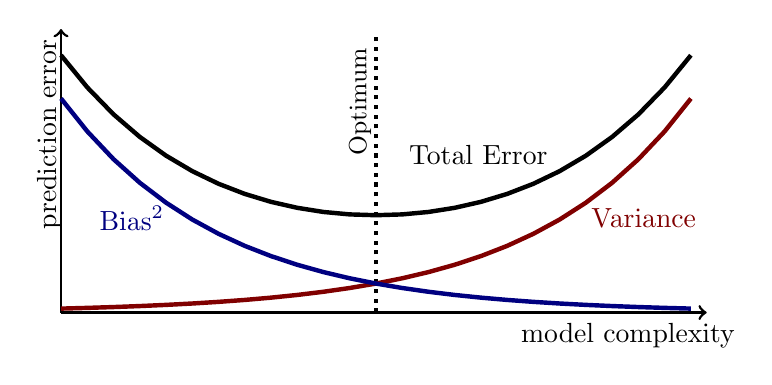
\begin{tikzpicture}
        \draw[->,line width=1pt,Black] (0,0) -> (0,3.6) node[left, rotate=90, yshift=0.15cm] {prediction error} ;
        \draw[->,line width=1pt,Black] (0,0) -> (8.2,0) node[below, xshift=-1cm] {model complexity} ;

        \draw[-,dotted,line width=1.5pt,Black] (4,0) -> (4,3.5) node[left, rotate=90, yshift=0.2cm] {\small{Optimum}};
        \draw[black, ultra thick, domain=-2:2] plot ({2*\x+4}, {exp(-\x-1)+exp(\x-1)+0.5});
        \node at (5.3, 2) {\textcolor{black}{Total Error}};
        \node at (7.4, 1.2) {\textcolor{red!50!black}{$\mathrm{Variance}$}};
        \node at (0.9, 1.2) {\textcolor{blue!50!black}{$\mathrm{Bias}^2$}};
        \draw[red!50!black, ultra thick, domain=-2:2] plot ({2*\x+4}, {exp(\x-1)});
        \draw[blue!50!black, ultra thick, domain=-2:2] plot ({2*\x+4}, {exp(-\x-1)});

      \end{tikzpicture}
    \end{center}
\end{frame}

\begin{frame}
    \frametitle{Model complexity}
    \begin{center}

      \textbf{Number of Degrees of freedom (NDF) of the model \\($\approx$ number of parameters)}
      \begin{itemize}
        \item Input dataset
        \begin{itemize}
          \item Reduce dimensionality
          \item Higher statistic
        \end{itemize}
        \item Hyperparameters (control NDF)
        \begin{itemize}
          \item Depth of the tree
          \item Minimum number of data points per leave
          \item Separation gain measure (entropy, gini-index)
          \item Optimized using search-algorithm
        \end{itemize}
        \item Regularization (reduce effective NDF)
        \begin{itemize}
          \item Prune overfitted branches of the tree
          \item Include tree structure in separation gain measure
          \item Ensemble methods
        \end{itemize}
      \end{itemize}

      \large{Always test on an independent test dataset in the end!}
    \end{center}
\end{frame}

